\begin{frame}
    \frametitle{Logistic Regression}
    \begin{columns}
        \column{.5\linewidth}
            \begin{itemize}
                \item Misnamed: Classification, not regression.
                \item Linear decision function: simple, easy to understand.
            \end{itemize}
        \column{.5\linewidth}
            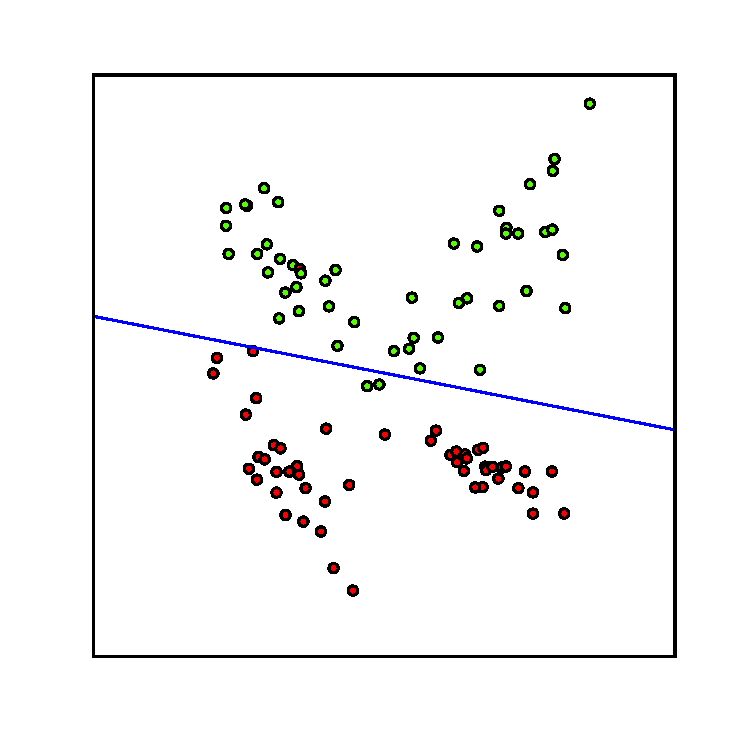
\includegraphics[width=1\linewidth]{logreg-pics/synthetic_line}\\

    \end{columns}
\end{frame}

\begin{frame}
    \frametitle{Example: Wisconsin Breast Cancer}
    \begin{columns}
        \column{.5\linewidth}
            \begin{itemize}
                \item Classify breast cancer samples in malign or benign.
                \item 700 Samples with 10 measurements each.
                \item We take only 3 measurements:
                    \begin{itemize}
                        \item Uniformity of Cell Size
                        \item Uniformity of Cell Shape
                        \item Single Epithelial Cell Size
                    \end{itemize}
                \item Training on 525, test on 175
                \item 97.1\% Accuracy
            \end{itemize}
        \column{.5\linewidth}
            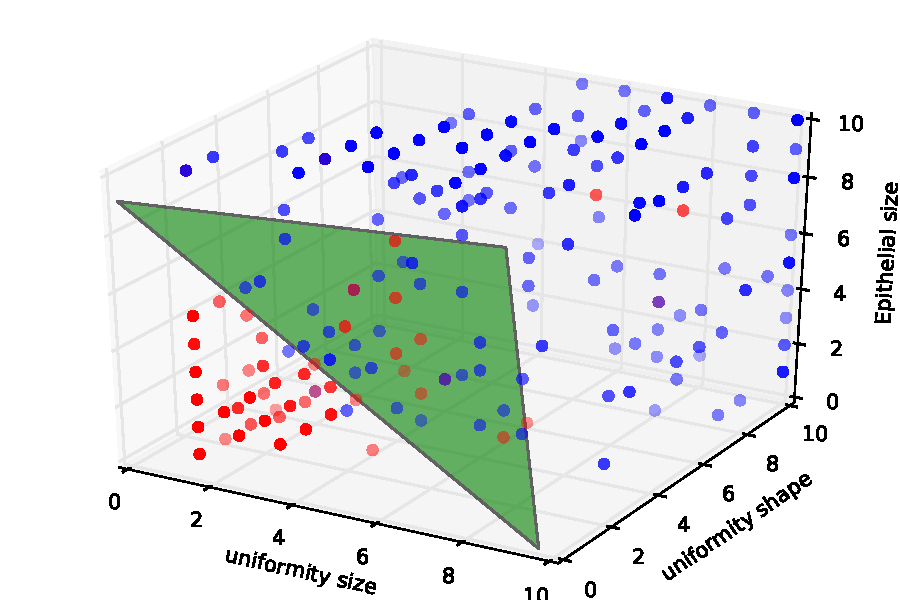
\includegraphics[width=1\linewidth]{logreg-pics/wisconsin_surface}
    \end{columns}

\end{frame}

\begin{frame}
    \frametitle{Mathematical Formulation I}
    \begin{columns}
        \column{.5\linewidth}
        \begin{itemize}
            \item For two classes $-1, +1$.
            \item Decision boundary given by hyperplane.
            \item Hyperplane defined by normal vector and offset:
                \begin{gather*}
                    y = \text{sign}(\left<w, x\right> + b)\\
                    w \in \mathbb{R}^n, b \in \mathbb{R}
                \end{gather*}
        \end{itemize}
        \column{.5\linewidth}
            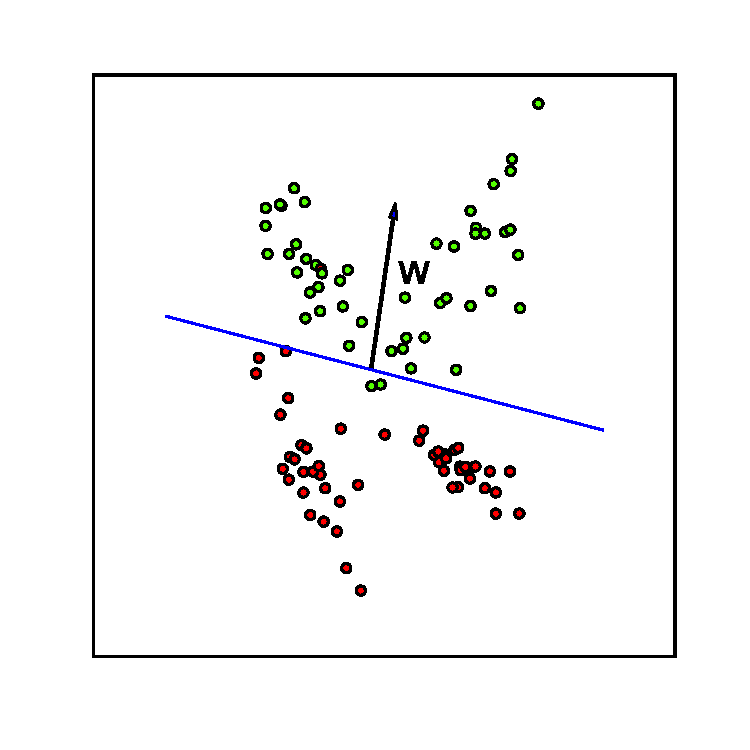
\includegraphics[width=1\linewidth]{logreg-pics/synthetic_line_w}\\

    \end{columns}
\end{frame}

\begin{frame}
    \frametitle{Mathematical Formulation II}
    \begin{columns}[T]
        \column{.5\linewidth}
            \begin{itemize}
                \item Relation to regression:
                    \begin{align*}
                        p(y=+1\,|\, x) = \text{logistic}(\left<w, x\right> + b)
                    \end{align*}
                \item As probabilities are between $0$ and $1$, the logistic function
                    squashes the regression result:
                    \begin{align*}
                         p(y=+1 \,|\, x) > 0.5 \Leftrightarrow \left <w, x \right> + b > 0
                     \end{align*}
            \end{itemize}
        \column{.4\linewidth}
            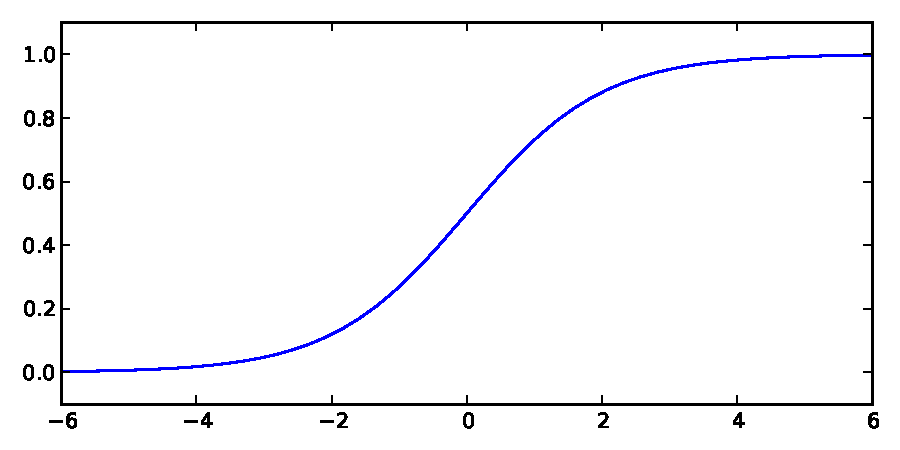
\includegraphics[width=.8\linewidth]{logreg-pics/logistic_sigmoid}\\
    \end{columns}
    \begin{itemize}
        \item Need to solve:
            \begin{align*}
                \min_w \sum_{i=0}^n \log(p(Y=y_i | x_i))
            \end{align*}
    \end{itemize}
\end{frame}


\begin{frame}
    \frametitle{Example: Classifying Insults I}
    \begin{columns}
        \column{.5\linewidth}
        \begin{itemize}
            \item Dataset: Forum posts / comments on social issues.
            \item Two classes: Insulting towards other posters / not insults.
            \item Training set: 4000 comments, test set: 2500 comments
            \item Features: Extract dictionary of all occuring words, count occurence per comment.
            \item Very high dimensional: 16.500
            \end{itemize}
        \column{.5\linewidth}
            \begin{beamercolorbox}[sep=1em,wd=5cm]{insult}
                \usebeamerfont{myserif}Either you are fake or extremely stupid\dots maybe both\dots\\
            \end{beamercolorbox}
            \vspace{1em}

            \begin{beamercolorbox}[sep=1em,wd=5cm]{noinsult}
                \usebeamerfont{myserif}i really don't understand your point. It seems that you are
                mixing apples and oranges.\\
            \end{beamercolorbox}
            \vspace{1em}

            \begin{beamercolorbox}[sep=1em,wd=5cm]{insult}
                \usebeamerfont{myserif}To engage in an intelligent debate with
                you is like debating to a retarded person.  It's useless.  It
                looks like you're bent on disregarding the efforts of the
                government.
            \end{beamercolorbox}
            \vspace{1em}

            \begin{beamercolorbox}[sep=1em,wd=5cm]{noinsult}
                \usebeamerfont{myserif}@jdstorm dont wish him injury but it happened on its OWN and i
                DOUBT he's injured, he looked embarrassed to me\\
            \end{beamercolorbox}
    \end{columns}
\end{frame}


\begin{frame}[t]
    \frametitle{Example: Classifying Insults II}
    \begin{columns}[t]
        \column{.4\linewidth}
            \begin{beamercolorbox}[sep=1em,wd=5cm]{insult}
                \usebeamerfont{myserif}Either you are fake or extremely stupid\dots maybe both\dots\\
            \end{beamercolorbox}
        \column{.4\linewidth}
            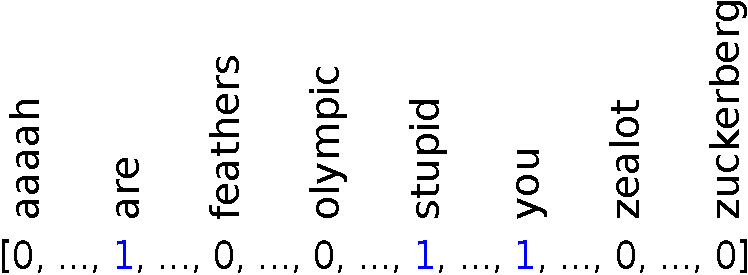
\includegraphics[width=.9\linewidth]{logreg-pics/bag_of_words-crop}\\
            
    \end{columns}
    \vspace{3mm}
    \begin{onlyenv}<2->
        Accuracy with logistic regression: 84.5\%\\
    \end{onlyenv}
    \vspace{3mm}
    \begin{onlyenv}<3>
        The largest coefficients (sign given by color):
        \begin{center}
            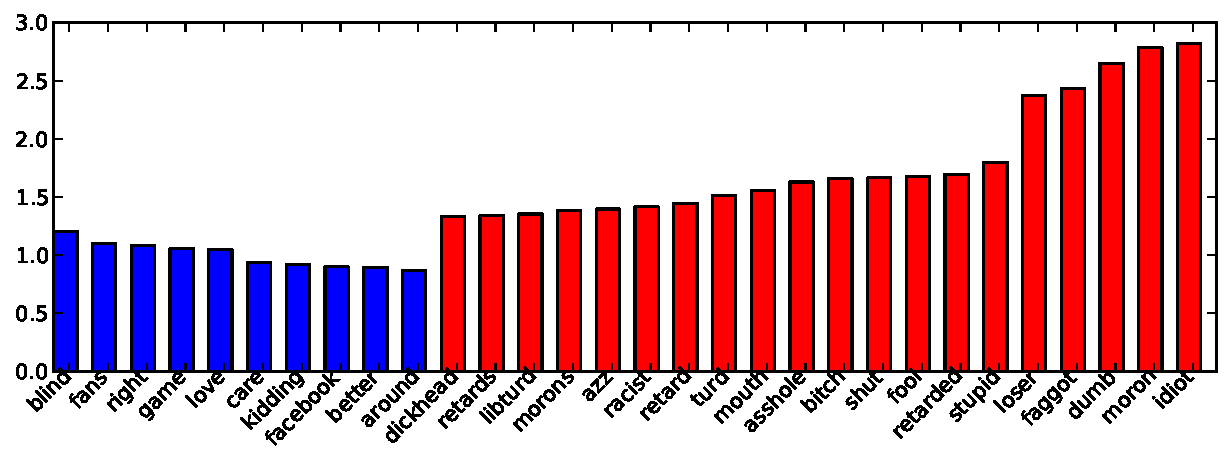
\includegraphics[width=.9\linewidth]{logreg-pics/bow_coef}
        \end{center}
    \end{onlyenv}
\end{frame}

%\begin{frame}
    %\frametitle{Logistic Regression -- Interactive}
    %\begin{itemize}
        %\item some 2D blobs dataset
        %\item  Breast Cancer dataset
        %\item  http://archive.ics.uci.edu/ml/datasets/Breast+Cancer+Wisconsin+%28Diagnostic%29
    %\end{itemize}
%\end{frame}
